\section{Evaluation}

\subsection{Datengenerierung}
\label{datagen}

Der Vorgang der Datengenerierung wurde nach dem in Abbildung \ref{fig:overview2} aufgezeigten Schema implementiert. Durch die Verwendung einer Custom Map (zu Deutsch: \textit{benutzerdefinierten Karte}), eine durch den in StarCraft~II mitgelieferten Editor modifizierte Spielfläche, können die beiden Armeen mit zufällig zusammengestellten Einheiten-Konstellationen generiert werden. Zu Beginn des Gefechts werden beide Armeen am gegenseitigen Ende der Karte erzeugt. Bevor die Armeen den Kampf beginnen, wird der Spiel-Zustand (Spieler IDs, Höhenkarte, Einheitentyp, etc.) in Form von mehreren Matrix-Repräsentationen gespeichert. Sobald eine der beiden Seiten keine Einheiten mehr hat gilt die Schlacht als beendet und die Armee, welche noch über Einheiten verfügt wird als Sieger betrachtet. Das Ergebnis wird als Integer-Wert gespeichert und im späteren Verlauf des Trainings zu einem One-Hot-Vektor transformiert. 

Die Armeen werden zufällig generiert, der Generierungsprozess läuft wie folgt ab: Zunächst wird für beide Armeen eine Rasse gewürfelt. Die Rasse bestimmt welche Einheiten die Armee erzeugen darf. Im Folgenden wird für jede Einheit durch einen Zufallszahlen-Generator die Anzahl der maximal zu erzeugenden Einheiten ermittelt. Die Anzahl der Einheit, welche insgesamt von einer Armee erzeugt werden dürfen ist auf eine zufällige Grenze zwischen 10 und 50 begrenzt. Es werden daher alle Werte der einzelnen Einheiten so reduziert, dass die Gesamtzahl der Einheiten in einer Armee diese Grenze nicht überschreitet. Da bei zu großen Unterschieden in der Armeegröße die Klassifizierung zu einer trivialen Aufgabe wird, wurde zusätzlich eine Versorgungs-Grenze implementiert. In StarCraft~II ist die Versorgungsgrenzer ein Wert, welcher die Größe der Armee eines Spieler begrenzt. Diese Grenze wird in dem Kontext der Datengenerierung genutzt um nur jene Gefechte zu erzeugen, in denen der Unterschied der Einheiten-Versorgung beider Armeen kleiner ist als ein definierter Grenzwert (in diesem Fall 5).

Abbildung \ref{fig:overview1} zeigt den Generierungsprozess in Gänze. Die Custom Map aus StarCraft~II generiert ein Gefecht mit passender Differenz an Einheiten-Versorgung und lässt dieses nach speichern des Spielzustands austragen. Dieser Vorgang wird vor dem Beenden der Custom Map 25 Mal ausgeführt. Mit Beenden der Custom Map werden alle Vorgänge auf der Karte, als Replay (zu Deutsch: \textit{Wiederholung}) gespeichert. Ein Replay enthält somit 25 Gefechte, welche alle einzeln ausgewertet werden. 

Die Entscheidung mehrere Gefechte auf einmal zu generieren wurde getroffen, da die Custom Map bei jedem Start das Spiel neu laden muss und somit der zeitliche Overhead bei Einzelgenerierung der Replays wesentlich größer wäre. Die Anzahl der in einem Replay generierten Gefechte wurde auf 25 gesetzt, da bei zu vielen Iterationen der Gefechtsgenerierung die Replay-Datei zu groß wurde und das Spiel beim Schließen der Custom Map abstürzte. Der Absturz resultierte in jedem Fall in einem Datenverlust. Bei 25 Gefechten pro Replay liegt die Absturzrate derzeit immer noch bei ca. 50\%, jedoch resultierte das weitere Senken der Gefechte pro Replay nicht in einem stabileren Generationsprozess. 

Die Generierung der Gefechte findet auf der schnellsten Spieleinstellung statt, damit in gleicher Zeit mehr Gefechte simuliert werden können. Dadurch ist es aktuell möglich in einem Zeitraum von acht Stunden ca. 250 valide (500 Generierungen inklusive der Abstürze) Replays zu produzieren, welche nach der Feature Extraktion (Zeitaufwand erneut ca. drei bis vier Stunden) in 6250 Samples resultieren. 

\newpage
\begin{figure}[H]
\thispagestyle{empty}
\centering
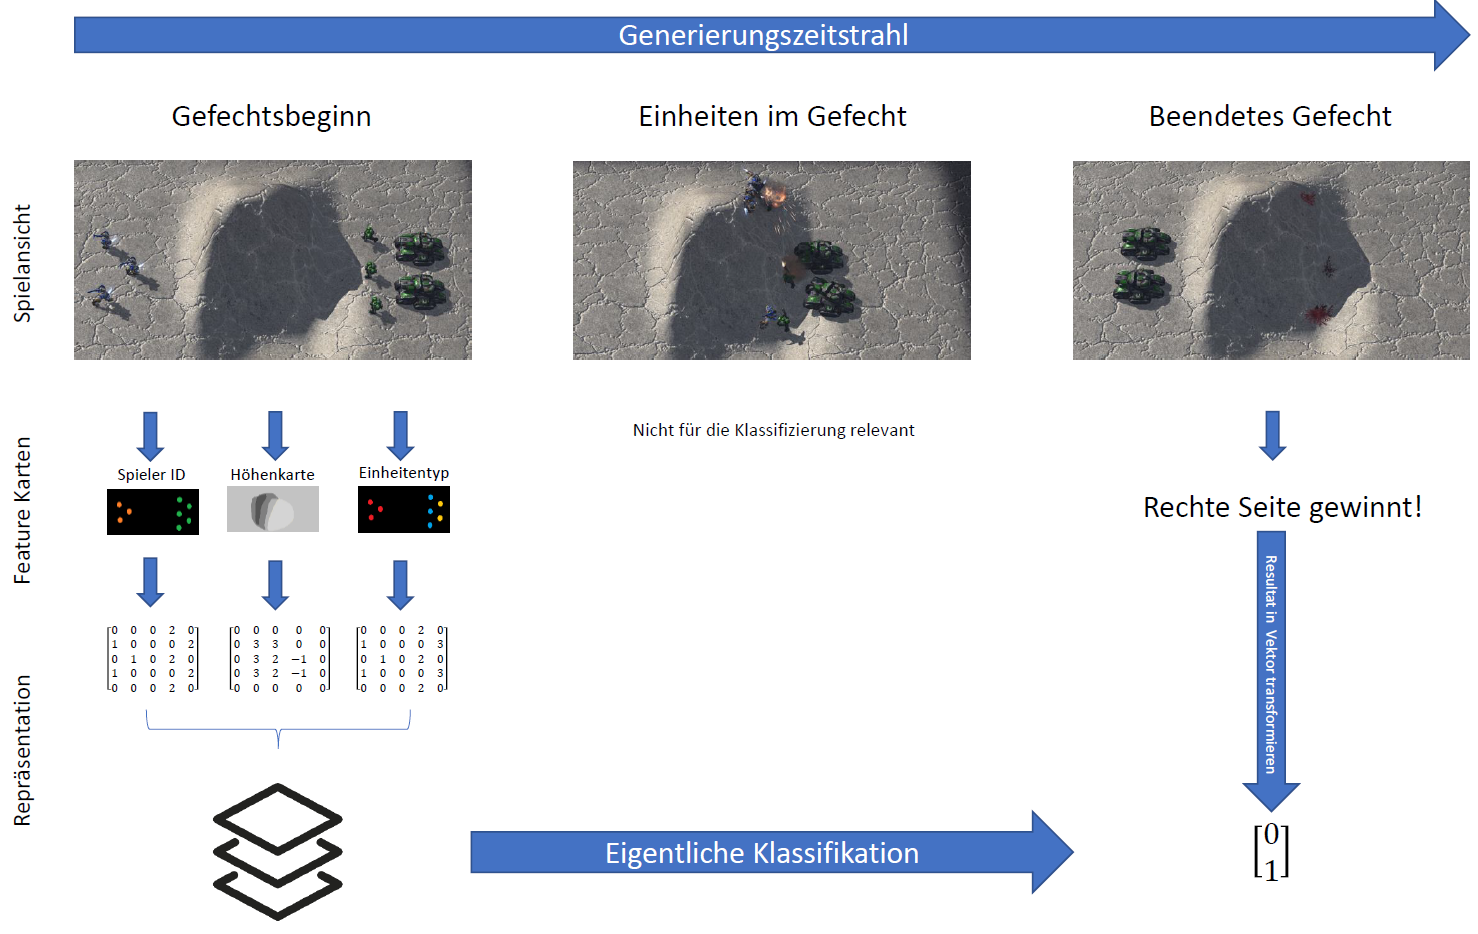
\includegraphics[angle=90,scale=0.6]{pictures/grafiken/Folie1}
\caption{Übersicht des Generierungsprozesses der Trainingsdaten}
\label{fig:overview2}
\end{figure}

\begin{figure}[H]
\thispagestyle{empty}
\centering
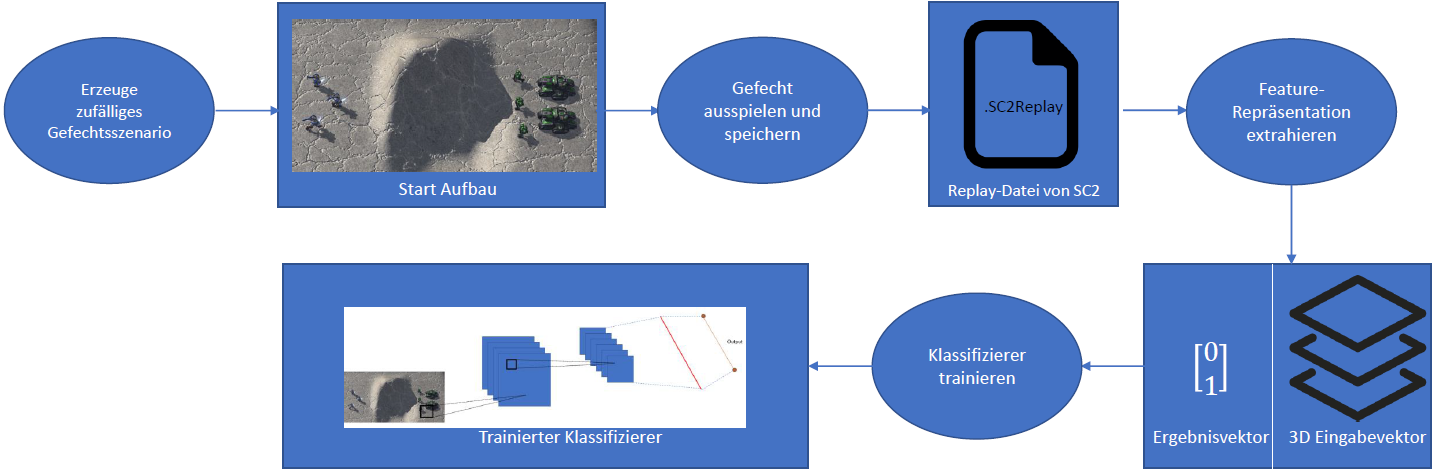
\includegraphics[angle=90,scale=0.6]{pictures/grafiken/Folie2}
\caption{Übersicht des Generierungsprozesses der Trainingsdaten}
\label{fig:overview1}
\end{figure}


\subsection{Resultate}
\label{Resultate}

\subsection{Auswertung}
\label{Auswertung}